\subsection{Популярность}

Результаты сравнения популярности приведены в таблице \ref{tab:popularity-comparison}.

\begin{table}[h!]
    \centering
    \begin{tabular}{lccc}
        \toprule
        \textbf{Фреймворк} & \textbf{Количество проектов} & \textbf{Количество звезд} \\
        \midrule
        EML & 258 & - \\
        MLX & 61 & 123 \\
        TYXML & 1200+ & 173 \\
        DHTML & 20 & 181 \\
        \bottomrule
    \end{tabular}
    \caption{Сравнение популярности}
    \label{tab:popularity-comparison}
\end{table}

\subsection{Покрытие}

Визуальное сравнение приведено в приложении \ref{apx:coverage}.
Его результаты таковы:

\begin{table}[h]
    \centering
    \caption{Сравнение покрытия}
    \label{tab:coverage-comparison}
    \begin{tabularx}{\linewidth}{l>{\raggedright\arraybackslash}X>{\raggedright\arraybackslash}XcXX}
        \toprule
        \textbf{Фреймворк} & \textbf{Комментарии} \\
        \midrule
        EML & \cellcolor{yellow!30} Изначальный шаблон теряется после работы препроцессора, результирующий код нечитабелен \\
        MLX & После препроцессора шаблон трансформируется в корректный OCaml код \\
        TYXML, DHTML & Не используется препроцессор, оригинальный код покрывается без потерь \\
        TYXML\% & Препроцессор в этом случае генерирует AST, которое в свою очередь обходится bisect-ом. Оригинальное представление кода сохраняется в покрытии \\
        \bottomrule
    \end{tabularx}
\end{table}

Как видно из сравнения, EML сильно проигрывает остальным шаблонизаторам, полностью теряя оригинальную структуру кода.



\subsection{Экосистема, дебаггинг и тестирование}

% // TODO доделать описание

\subsection{Документация}

% // TODO доделать описание

\subsection{Поддержка UTF-8}

Все фреймворки поддерживают UTF-8.
После препроцессинга (для EML и MLX) русские символы заменяются их представлением в UTF-8.
В случае TyXML\% первый символ просто неправильно отображается в сгенерированном покрытии, хотя код страницы получающийся в результате работы функции корректен.
В связи с этим, сделан вывод что это ошибка на стороне bisect\_ppx, которая была отрепортирована % // TODO: отрепортировать
Примеры приведены на рис. \ref{fig:utf8}.

\begin{figure}[ht!]
    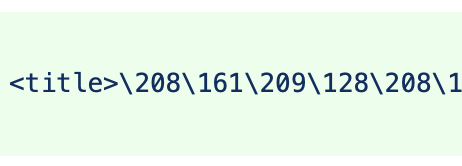
\includegraphics[width=.3\textwidth]{utf8eml}\hfill
    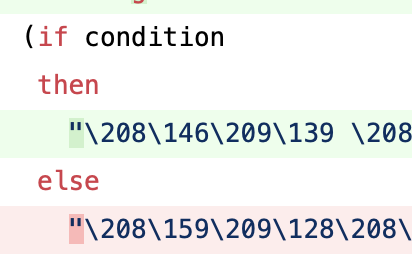
\includegraphics[width=.3\textwidth]{utf8mlx}\hfill
    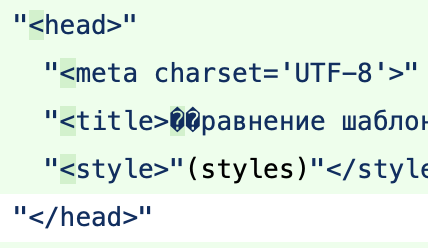
\includegraphics[width=.3\textwidth]{utf8tyxml}
    \caption{EML, экранированные UTF-8 символы}
    \caption{MLX, экранированные UTF-8 символы}
    \caption{TyXML, ошибка отображения первых символов в строке}
    \label{fig:utf8}
\end{figure}
